\chapter{Arhitektura i dizajn sustava}
		
		\textbf{\textit{dio 1. revizije}}\\

		\textit{ Potrebno je opisati stil arhitekture te identificirati: podsustave, preslikavanje na radnu platformu, spremišta podataka, mrežne protokole, globalni upravljački tok i sklopovsko-programske zahtjeve. Po točkama razraditi i popratiti odgovarajućim skicama:}
	\begin{itemize}
		\item 	\textit{izbor arhitekture temeljem principa oblikovanja pokazanih na predavanjima (objasniti zašto ste baš odabrali takvu arhitekturu)}
		\item 	\textit{organizaciju sustava s najviše razine apstrakcije (npr. klijent-poslužitelj, baza podataka, datotečni sustav, grafičko sučelje)}
		\item 	\textit{organizaciju aplikacije (npr. slojevi frontend i backend, MVC arhitektura) }		
	\end{itemize}

	
		

		

				
		\section{Baza podataka}
			
			\textbf{\textit{dio 1. revizije}}\\
			
		\text Za potrebe našeg sustava koristit ćemo relacijsku bazu podataka koja svojom strukturom olakšava modeliranje stvarnog svijeta. Gradivna jedinka baze je relacija, odnosno tablica koja je definirana svojim imenom i skupom atributa. Zadaća baze podataka je brza i jednostavna pohrana, izmjena i dohvat podataka za daljnju obradu.
		\text Baza podataka se sastoji od idućih entiteta:
		\begin{packed_item}
			
			\item Korisnik
			\item Spasilac
			\item Stanica
			\item Akcija
			\item Poziv na akciju
			\item Galerija akcije
			\item Zadatak
			\item Komentari akcije
			\item Ruta

		\end{packed_item}
		
			\subsection{Opis tablica}

				\textbf {Korisnik} \text Ovaj entitet sadrži općenite informacije o svim korisnicima aplikacije Sadrži atribute: Korisničko ime, fotografiju,
								hash lozinke, ime, prezime, broj mobitela korisnika, e-mail, ulogu i status potvrde registracije. Ovaj entitet je u vezi
								\textit{One-to-one} sa entitetom Spasilac preko atributa korisničko ime, u vezi \textit{One-to-many} sa entitetom 										Akcija preko atributa korisničko ime dispečera te je u vezi \textit{One-to-many} sa entitetom Zadatak preko atributa
								korisničko ime dispečera. 
				
				
				\begin{longtblr}[
					label=none,
					entry=none
					]{
						width = \textwidth,
						colspec={|X[6,l]|X[6, l]|X[20, l]|}, 
						rowhead = 1,
					} %definicija širine tablice, širine stupaca, poravnanje i broja redaka naslova tablice
					\hline \multicolumn{3}{|c|}{\textbf{Korisnik}}	 \\ \hline[3pt]
					\SetCell{LightGreen}Korisnicko ime & VARCHAR & jedinstveno korisničko ime  	 	\\ \hline
					Fotografija	& LONGBLOB & Fotografija korisnika  	\\ \hline
					Hash lozinke & VARCHAR & Hash lozinke korisnika  	\\ \hline 
					Ime & VARCHAR & Ime korisnika  	\\ \hline
					Prezime & VARCHAR & Prezime korisnika  	\\ \hline
					Broj mobitela & VARCHAR & Broj mobitela korisnika  	\\ \hline 
					e-mail & VARCHAR & e-mail korisnika  \\ \hline 
					Uloga & VARCHAR	& Uloga korisnika		\\ \hline
					Potvrđen & BOOLEAN & Status registracije korisnika  
				\end{longtblr}



				\textbf {Spasilac} \text Ovaj entitet sadrži sve važne informacije o spasiocima. Sadrži atribute: Korisničko ime, osposobljenje, lokacija, 									  zauzetost, idAkcija i idStanice kojoj spasilac pripada. Ovaj entitet je u vezi \textit{One-to-one} sa entitetom Korisnik preko 							  atributa Korisničko ime, u vezi \textit{One-to-many} sa entitetom Poziv na akciju preko atributa Korisničko ime spasioca, u 							  vezi \textit{One-to-Many} sa entitetom Zadatak preko atributa Korisničko ime spasioca, u vezi \textit{One-to-Many} sa 									  entitetom Komentari Akcije preko atributa Korisničko ime te u vezi \textit{One-to-one} sa entitetom Akcija preko atributa 									  idAkcije.
				
				
				\begin{longtblr}[
					label=none,
					entry=none
					]{
						width = \textwidth,
						colspec={|X[6,l]|X[6, l]|X[20, l]|}, 
						rowhead = 1,
					} %definicija širine tablice, širine stupaca, poravnanje i broja redaka naslova tablice
					\hline \multicolumn{3}{|c|}{\textbf{Spasilac}}	 \\ \hline[3pt]
					\SetCell{LightGreen}Korisničko ime & VARCHAR	&  	Korisničko ime spasioca  	\\ \hline
					Osposobljenje	& VARCHAR &  Osposobljenje spasioca 	\\ \hline 
					Lokacija & VARCHAR &  Lokacija spasioca \\ \hline 
					Zauzetost & BOOLEAN	&  Status zauzetosti spasioca 		\\ \hline 
					\SetCell{LightBlue} idAkcije	& VARCHAR & id akcije na kojoj se spasilac trenutno nalazi  	\\ \hline 
					\SetCell{LightBlue} idStanice	& VARCHAR &  id stanice kojoj spasilac pripada 	\\ \hline 
				\end{longtblr}
			
				

				\textbf{Akcija} \text Ovaj entitet sadrži sve važne informaije o akciji. Sadrži atribute: idAkcije, adresu, gotova, i opis akcije. Ovaj entitet je u 						             vezi \textit{One-to-one} sa entitetom Spasilac preko atributa idAkcije, u vezi \textit{One-to-many} sa entitetom Galerija 							     akcije preko atributa idAkcije, u vezi \textit{One-to-many} sa entitetom Komentari akcije preko atributa idAkcije te u 									     vezi \textit{One-to-many} sa entitetom Poziv na akciju preko atributa idAkcije.
				
				
				\begin{longtblr}[
					label=none,
					entry=none
					]{
						width = \textwidth,
						colspec={|X[6,l]|X[6, l]|X[20, l]|}, 
						rowhead = 1,
					} %definicija širine tablice, širine stupaca, poravnanje i broja redaka naslova tablice
					\hline \multicolumn{3}{|c|}{\textbf{Akcija}}	 \\ \hline[3pt]
					\SetCell{LightGreen}idAkcije & INT	&  	id akcije  	\\ \hline
					Adresa	& VARCHAR &  adresa  	\\ \hline 
					Gotova & BOOLEAN &  oznaka završetka akcije \\ \hline 
					Opis akcije & VARCHAR	&  kratak opis akcije		\\ \hline 
				\end{longtblr}

				
				\textbf{Poziv na akciju} \text Ovaj entitet sadrži sve važne informaije o pozivu na akciju pojedinačnom spasiocu. Sadrži atribute: Korisničko 										  ime spasioca, id akcije, način sudjelovanja spasioca, hitnost, odgovor spasioca, komentar i korisničko ime 											  dispečera. Ovaj entitet je u vezi \textit{Many-to-many} sa entitetom Spasilac preko atributa Korisničko ime 											  spasioca, u vezi \textit{Many-to-many} sa entitetom Korisnik preko atributa Korisničko ime dispečera te u vezi 											  \textit{One-to-one} sa entitetom Akcija preko atributa idAkcije.
				
				
				\begin{longtblr}[
					label=none,
					entry=none
					]{
						width = \textwidth,
						colspec={|X[6,l]|X[6, l]|X[20, l]|}, 
						rowhead = 1,
					} %definicija širine tablice, širine stupaca, poravnanje i broja redaka naslova tablice
					\hline \multicolumn{3}{|c|}{\textbf{Poziv na akciju}}	 \\ \hline[3pt]
					\SetCell{LightGreen}Korisničko ime spasioca & VARCHAR	&  	Korisničko ime spasioca kojem je poslan poziv  	\\ \hline
					\SetCell{LightGreen}idAkcije & INT	&  	id akcije za koju se šalje poziv  	\\ \hline
					Način sudjelovanja	& VARCHAR & način sudjelovanja spasioca  	\\ \hline 
					Hitnost & INT & razina hitnosti  \\ \hline 
					Odgovor spasioca & BOOLEAN	&  Prihvat poziva ili odbijanje\\ \hline
					Komentar	& VARCHAR & komentar dispečera  	\\ \hline  
					\SetCell{LightBlue} Korisničko ime dispečera	& VARCHAR &   	Korisničko ime dispečera koji je poslao poziv\\ \hline 
				\end{longtblr}
				
				\textit{Svaku tablicu je potrebno opisati po zadanom predlošku. Lijevo se nalazi točno ime varijable u bazi podataka, u sredini se nalazi tip podataka, a desno se nalazi opis varijable. Svjetlozelenom bojom označite primarni ključ. Svjetlo plavom označite strani ključ}
				
				
				\begin{longtblr}[
					label=none,
					entry=none
					]{
						width = \textwidth,
						colspec={|X[6,l]|X[6, l]|X[20, l]|}, 
						rowhead = 1,
					} %definicija širine tablice, širine stupaca, poravnanje i broja redaka naslova tablice
					\hline \multicolumn{3}{|c|}{\textbf{korisnik - ime tablice}}	 \\ \hline[3pt]
					\SetCell{LightGreen}IDKorisnik & INT	&  	Lorem ipsum dolor sit amet, consectetur adipiscing elit, sed do eiusmod  	\\ \hline
					korisnickoIme	& VARCHAR &   	\\ \hline 
					email & VARCHAR &   \\ \hline 
					ime & VARCHAR	&  		\\ \hline 
					\SetCell{LightBlue} primjer	& VARCHAR &   	\\ \hline 
				\end{longtblr}
				
				
			
			\subsection{Dijagram baze podataka}
				\textit{ U ovom potpoglavlju potrebno je umetnuti dijagram baze podataka. Primarni i strani ključevi moraju biti označeni, a tablice povezane. Bazu podataka je potrebno normalizirati. Podsjetite se kolegija "Baze podataka".}

				\begin{figure}[H]
					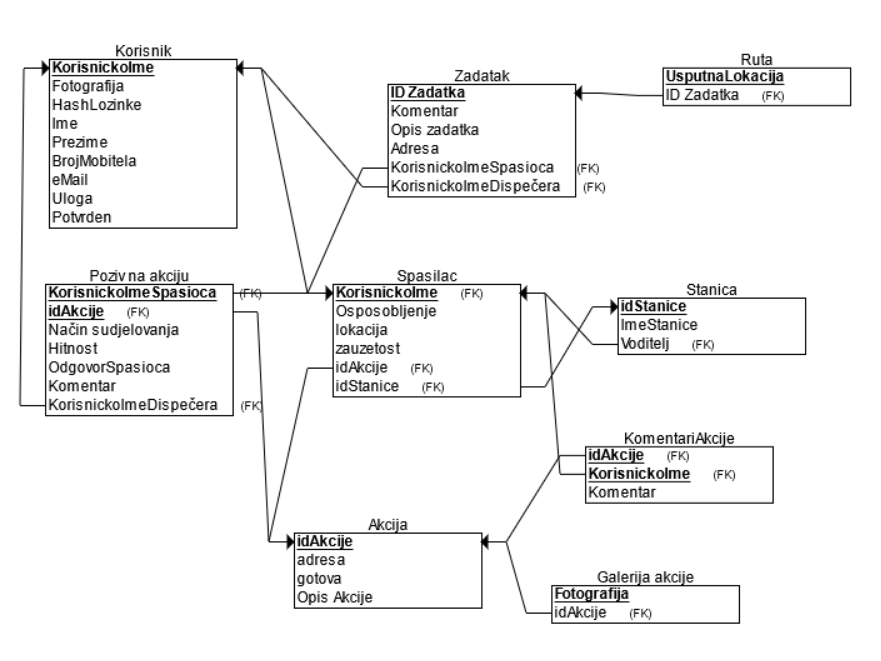
\includegraphics[scale=0.4]{slike/ModelBazePodataka.png} %veličina slike u odnosu na originalnu datoteku i pozicija slike
					\centering
					\caption{ER dijagram baze podataka}
					\label{fig:promjene}
				\end{figure}
			
			\eject
			
			
		\section{Dijagram razreda}
		
			\textit{Potrebno je priložiti dijagram razreda s pripadajućim opisom. Zbog preglednosti je moguće dijagram razlomiti na više njih, ali moraju biti grupirani prema sličnim razinama apstrakcije i srodnim funkcionalnostima.}\\
			
			\textbf{\textit{dio 1. revizije}}\\
			\begin{figure}[H]
				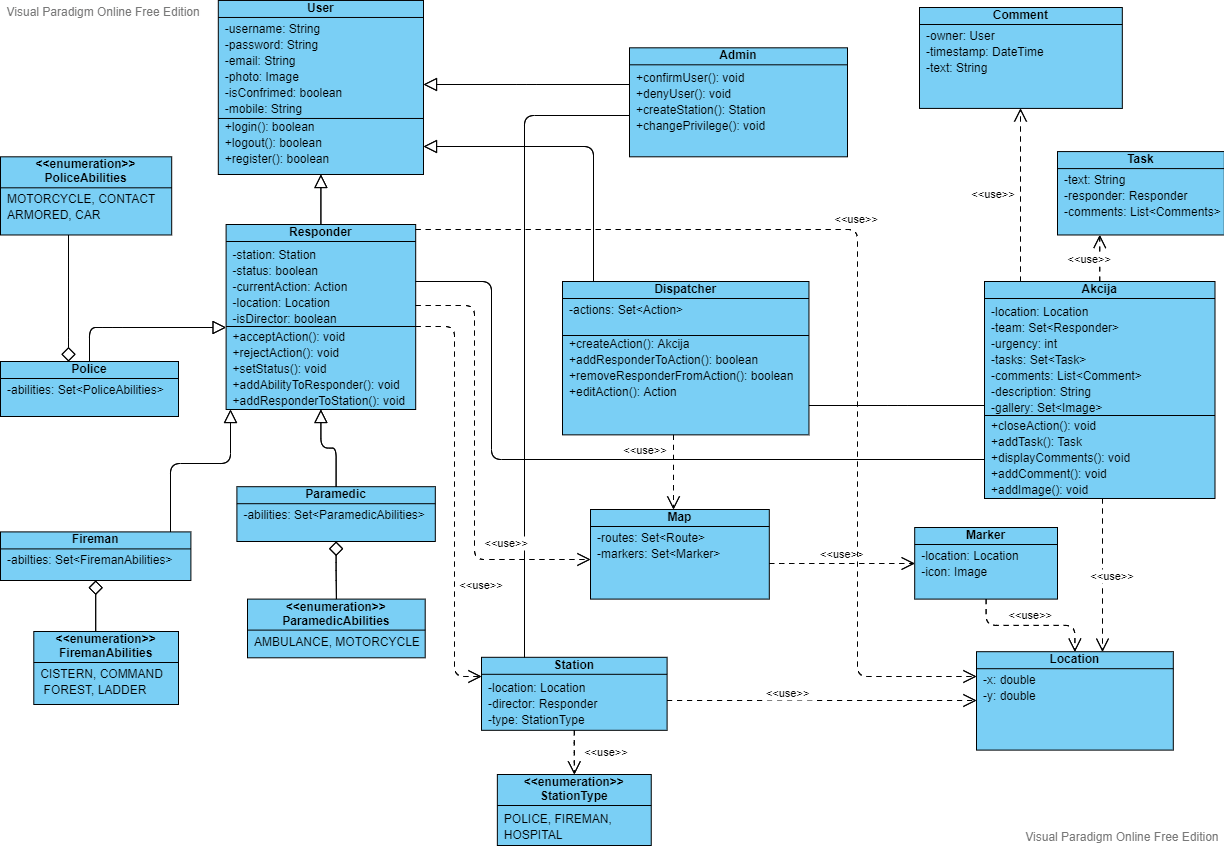
\includegraphics[scale=0.4]{slike/classes.PNG}
				\centering
				\caption{Dijagram razreda}
				\label{fig:razredi}
			\end{figure}
		
			\textit{Prilikom prve predaje projekta, potrebno je priložiti potpuno razrađen dijagram razreda vezan uz \textbf{generičku funkcionalnost} sustava. Ostale funkcionalnosti trebaju biti idejno razrađene u dijagramu sa sljedećim komponentama: nazivi razreda, nazivi metoda i vrste pristupa metodama (npr. javni, zaštićeni), nazivi atributa razreda, veze i odnosi između razreda.}\\
			
			\textbf{\textit{dio 2. revizije}}\\			
			
			\textit{Prilikom druge predaje projekta dijagram razreda i opisi moraju odgovarati stvarnom stanju implementacije}
			
			
			
			\eject
		
		\section{Dijagram stanja}
			
			
			\textbf{\textit{dio 2. revizije}}\\
			
			\textit{Potrebno je priložiti dijagram stanja i opisati ga. Dovoljan je jedan dijagram stanja koji prikazuje \textbf{značajan dio funkcionalnosti} sustava. Na primjer, stanja korisničkog sučelja i tijek korištenja neke ključne funkcionalnosti jesu značajan dio sustava, a registracija i prijava nisu. }
			
			
			\eject 
		
		\section{Dijagram aktivnosti}
			
			\textbf{\textit{dio 2. revizije}}\\
			
			 \textit{Potrebno je priložiti dijagram aktivnosti s pripadajućim opisom. Dijagram aktivnosti treba prikazivati značajan dio sustava.}
			
			\eject
		\section{Dijagram komponenti}
		
			\textbf{\textit{dio 2. revizije}}\\
		
			 \textit{Potrebno je priložiti dijagram komponenti s pripadajućim opisom. Dijagram komponenti treba prikazivati strukturu cijele aplikacije.}